\documentclass{chi2009}
\usepackage{times}
\usepackage{url}
\usepackage{graphicx}
\usepackage{color}
\usepackage[pdftex]{hyperref}
\hypersetup{%
  pdftitle={Herbie Interactive Visualization},
  pdfauthor={Alex Sanchez-Stern},
}
\begin{document}
\special{papersize=8.5in,11in}
\setlength{\paperheight}{11in}
\setlength{\paperwidth}{8.5in}
\setlength{\pdfpageheight}{\paperheight}
\setlength{\pdfpagewidth}{\paperwidth}

\title{Herbie Interactive Visualization}
\author{Alex Sanchez-Stern}

\maketitle

\begin{abstract}
  Floating point rounding errors are notoriously difficult to detect and
  debug. By identifying the input regions for which error is high, and
  applying rewrites and taylor expanding at focused locations, the
  Herbie tool can automatically improve the accuracy of floating point
  expressions. But this process is complex for humans to understand a
  replicate. The Herbie Interactive Exploration allows users to get
  inside the inner workings of Herbie, and learn how it improves the
  accuracy of floating point programs, as well as how they might improve
  accuracy by hand.
\end{abstract}

\section{Introduction}
Many applications, in domains as diverse as scientific computing,
real-time simulation, and graphics, depend on the use of floating
point computations to approximate real number
computation. Unfortunately, due to the finite nature of the floating
point representation, computations using floating point numbers are
subject to rounding error, where a real number result is rounded to
the closest floating point number, losing some of it's precision. The
total error resulting from the accumulation of rounding error can grow
arbitrarily, and the resulting error is difficult to detect and
debug~\cite{berkeley00-needle-like, kahan-java-hurts,
  cse14-practical-fp}.

The Herbie tool, a tool under development at the University of
Washington, attempts to address these floating point issues. It does
so by automatically synthesizing floating point programs whose
numerical behavior most closely matches the behavior of a given
real-number formula. Unfortunately, while the project can successfully
produce more accurate implementations of a variety of formulas, it's
behavior is rather unintuitive. Herbie tends to produce programs for
which it is unclear how they connect to the supplied real-number
formula. Even when Herbie produces relatively straightforward output,
it is not always clear how it got there.

The Herbie Interactive Visualization hopes bridge the gap between
Herbie's ability to improve programs and the users knowledge about
floating point behavior and improvement, by providing an interface
through which users can visualize and control Herbie's improvement
process. Users can use this tool both as an alternative way to
directly improve their floating point code, and as a way to better
understand floating point behavior.

The rest of the paper is organized as follows. In
Section~\ref{sec:related}, I'll overview other works in the area of
floating point accuracy issues, as well as another tool that hopes to
teach users about unintuitive floating point behavior. In
Section~\ref{sec:methods}, I'll overview the design and algorithms of
the Herbie Interactive Visualization tool. In
Section~\ref{sec:results}, I'll show the resulting tool. In
Section~\ref{sec:discussion}, I'll discuss some insights found from
use of the tool, and finally, in Section~\ref{sec:future-work}, I'll
discuss how this work could be extended and improved.

\section{Related Work}
\label{sec:related}

There is much work demonstrating the unintuitive behavior of floating
point programs~\cite{berkeley00-needle-like, kahan-java-hurts,
  cse14-practical-fp}, but very few projects to attempt to educate
programmers about this behavior and empower them to understand
floating point behavior.

FPAvisual, a tool developed by Yi Gu et. al. does attempt to teach
students of programming about the unintuitive behavior of floating
point programs~\cite{fpavisual}. It does this by presenting four
specialized cases in which floating point behavior deviates from
expectation, as four seperate modes of the application.

The first, called ``Roots'', computes the quadratic formula using both
exact and floating point arithmetic, for user supplied inputs. Several
intermediary steps are also displayed, and the user can see the error
of each by manually comparing it to the correct result, also shown.

The second, called ``Pentagon'', displays a pentagon to the user, and
allows them to perform operations which should cancel each other out,
but due to rounding error produce slightly different pentagons. By
repeatedly applying these operations, the user can see the deviation
from the correct result grow.

In ``Associative Law'', the user is shown the graphs of five formulas
which are identical besides for slightly different associations. As
the formulas are recursive, the error can be visually seen to
accumulate.

Finally, in ``Sine Function'', the user is shown an error behavior
graph, much like the one produced by Herbie Interactive Visualization,
for different implementations of the $\sin{x}$ function. The different
implementations can be hidden or unhidden, and compared visually.

Though both attempt to teach users about floating point behavior, the
FPAvisual and the Herbie Interactive Visualization have some key
differences. Firstly, while FPAvisual allows detailed exploration of
specific examples, Herbie Interactive Visualization allows users to
enter the formulas they care about, merging learning and utility as
the users can apply the tool directly to their work. Secondly, Herbie
Interactive Visualization is more focused on teaching the user about
\textbf{improving} their floating point code, while FPAvisual focuses
on teaching them about the pitfalls in it's behavior.

\section{Methods}
\label{sec:methods}
The visualization was constructed in two parts: the visual front-end,
running in the browser on top of the d3 framework, and the back-end, a
Herbie session running on the server. There is also an input page
which uses MathJS to parse input formulas into s-expressions. The
back-end serves the input, improvement, and results pages, but other
than that only communicates to the front-end through GET parameters
and AJAX json requests.

Locations of error are already identified as part of Herbie's
improvement process, so for this visualization the existing locations
are pruned down to the top two, and then presented to the user for
improvement.

More difficult is the problem of deciding which axis to use to display
the error behavior to the user. The intuition is that the user would
prefer to see the axis on which the error best ``clumps'' into regions
representing the different sources of error. To accomplish this, we
take every sampled point and it's error, and filter out all points for
which the original formula has less than ten bits of error. Then, we
cluster these points into five clusters using the k-means clustering
algorithm. Finally, we measure the fitness of each clustering by
adding the squares of the distances of each point from it's cluster
mean. The axis on which this clustering returns the smallest aggregate
distance is chosen to represent error to the user.

Once an axis has been chosen, we must now identify regions for which
each highlighted operation contributes significantly to the
error. Since Herbie already includes a mechanism for assessing the
error of each operation, it is trivial to find the errors of
highlighted operations at each point. But finding ranges in these
points which are ``bad'' is another problem entirely. In the end, I
settled on picking the points with the highest error, and then walking
outwards from those points to form ranges.

Finally, plotting the error directly would result in a fairly jerky
graph which would obscure the larger trends of error. Instead, we
bucket points to create a smoothed line which clearly shows the
high-level error behavior.

Given the information we have so far, we can show the user a graph of
the error of the program, with ranges of high error highlighted
corresponding to the operations they correspond to. Next, we allow the
user to pick an operation at which they would like to focus
improvements for the iteration.

In this next phase, we must provide improved candidates which the user
can choose to keep or not. But Herbie itself produces on the order of
twenty candidates for each highlighted location, and showing all these
to the user could potentially overwhelm them. Instead, we pick the
three candidates of the ones generated which have the best error
behavior on the points that the original did badly on. This appears to
mostly pick candidates that are useful.

Next, we display the error graph of the branching combination of all
candidates selected so far, as well as the individual candidates and
their error graphs. We additionally plot the combination error on each
of the individual candidate graphs, so that the user can easily
compare how each candidate's error relates to the error of the
branching combination, and can easily see where each candidate was
used by looking to where it's like matches up with the line of the
combination.

From here the user can select a candidate to keep improving it, or go
to a final page where the branches will be recomputed with higher
accuracy and displayed to the user.

\section{Results}
\label{sec:results}

\begin{figure}
  \centering
  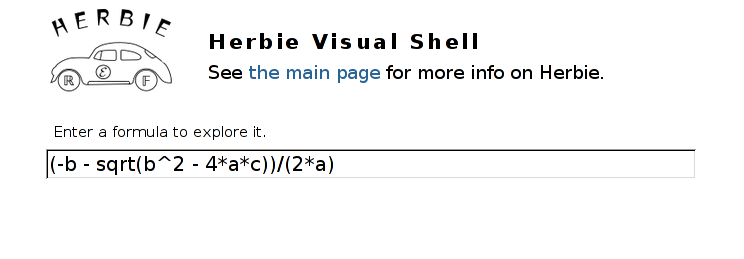
\includegraphics[width=.5\textwidth]{../../images/enter_formula_screen.png}
  \caption{The formula entry screen for the Herbie Interactive
    Visualization. Formulas can be entered in a c-like syntax, and are
    parsed client-side with MathJS.}
  \label{fig:enter-formula}
\end{figure}

\begin{figure}
  \centering
  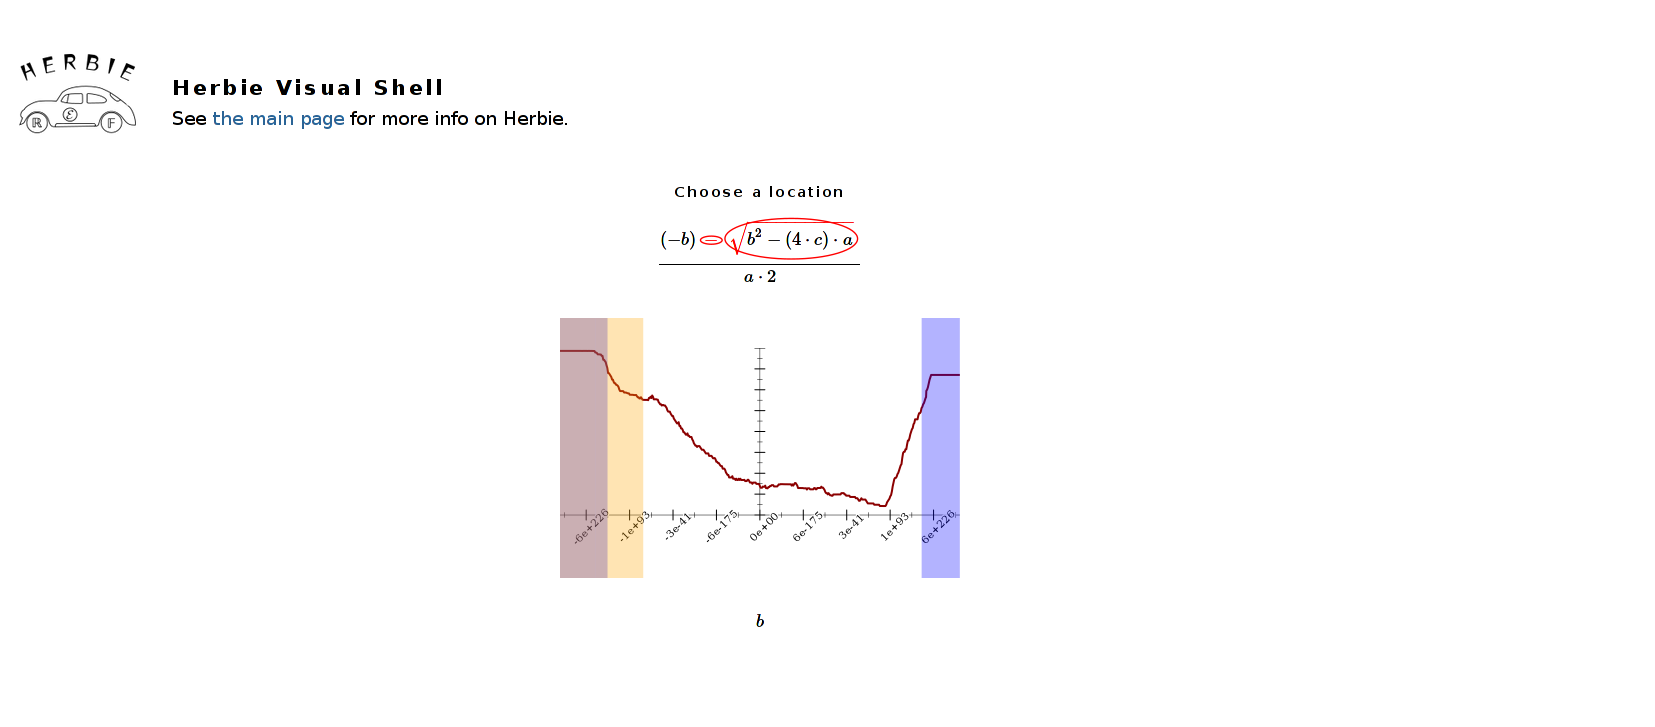
\includegraphics[width=.5\textwidth]{../../images/select_location_screen.png}
  \caption{The first phase of improvement. Here the user is shown the
    error behavior of the program, and selects an operation to
    rewrite. Notice that regions which have been identified as being
    caused by certain operations are highlighted, with one color per
    operation. Mousing over the operations expands their highlights so
    the user can easily connect operation to highlight.}
  \label{fig:select-loc}
\end{figure}

\begin{figure}
  \centering
  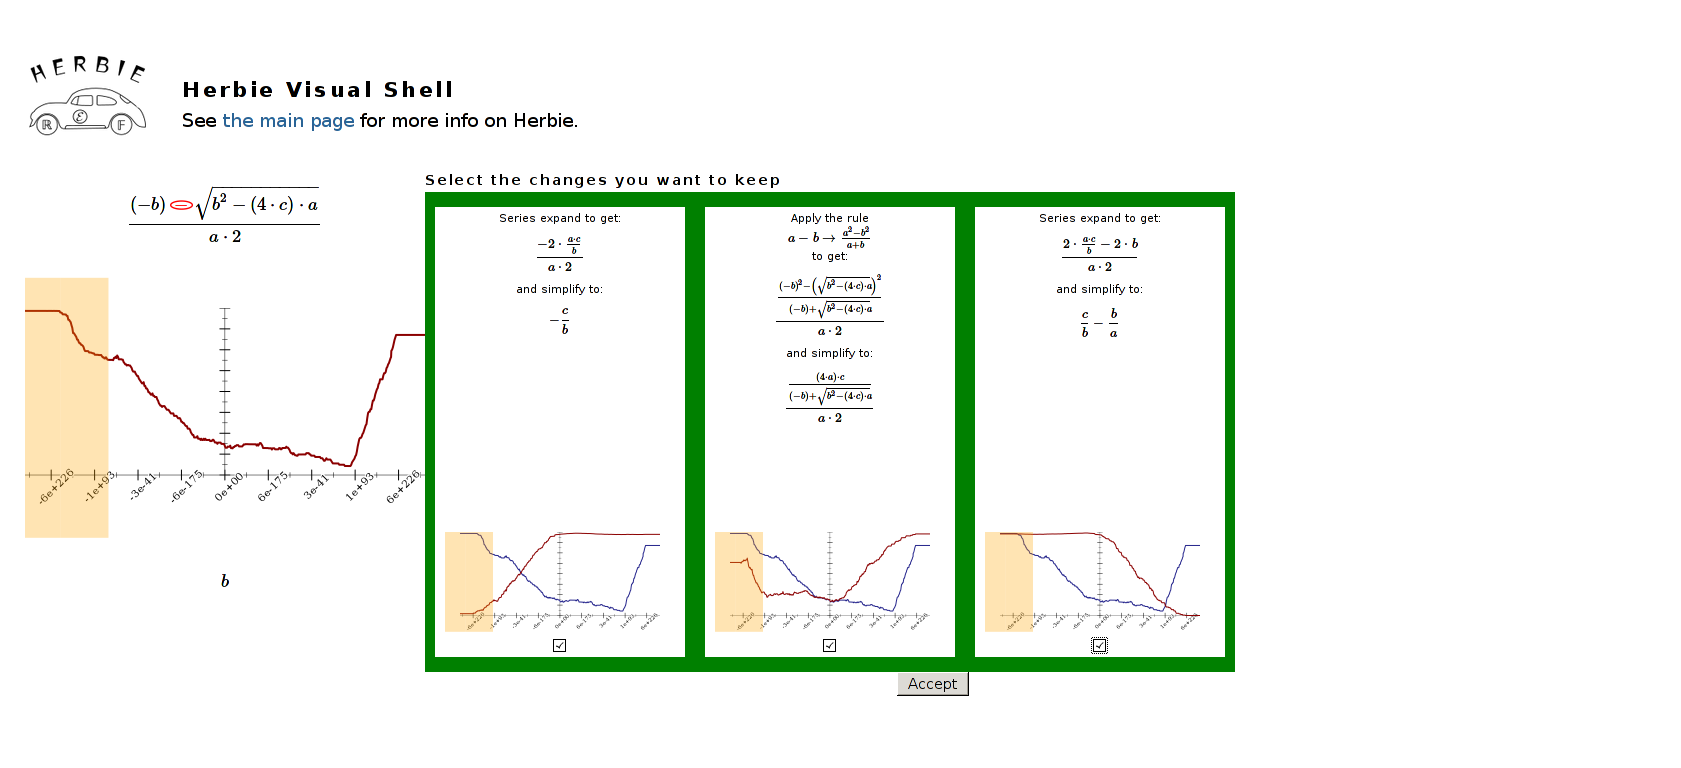
\includegraphics[width=.5\textwidth]{../../images/select_children_screen.png}
  \caption{The second phase of improvement. Here the user is presented
    with new candidate programs, resulting from Herbie attempting to
    rewrite the selected operation. These three are pruned from a
    larger set, since it seems that including more candidates would be
    distracting and would not help the user understand their
    program. For each candidate, the user is shown the rewrite steps
    which result in that candidate, and a graph of the error of that
    candidate compared to the error of the original program. In
    subsequent iterations, the error of each candidate is compared to
    the best combination found so far.}
  \label{fig:select-children}
\end{figure}

\begin{figure}
  \centering
  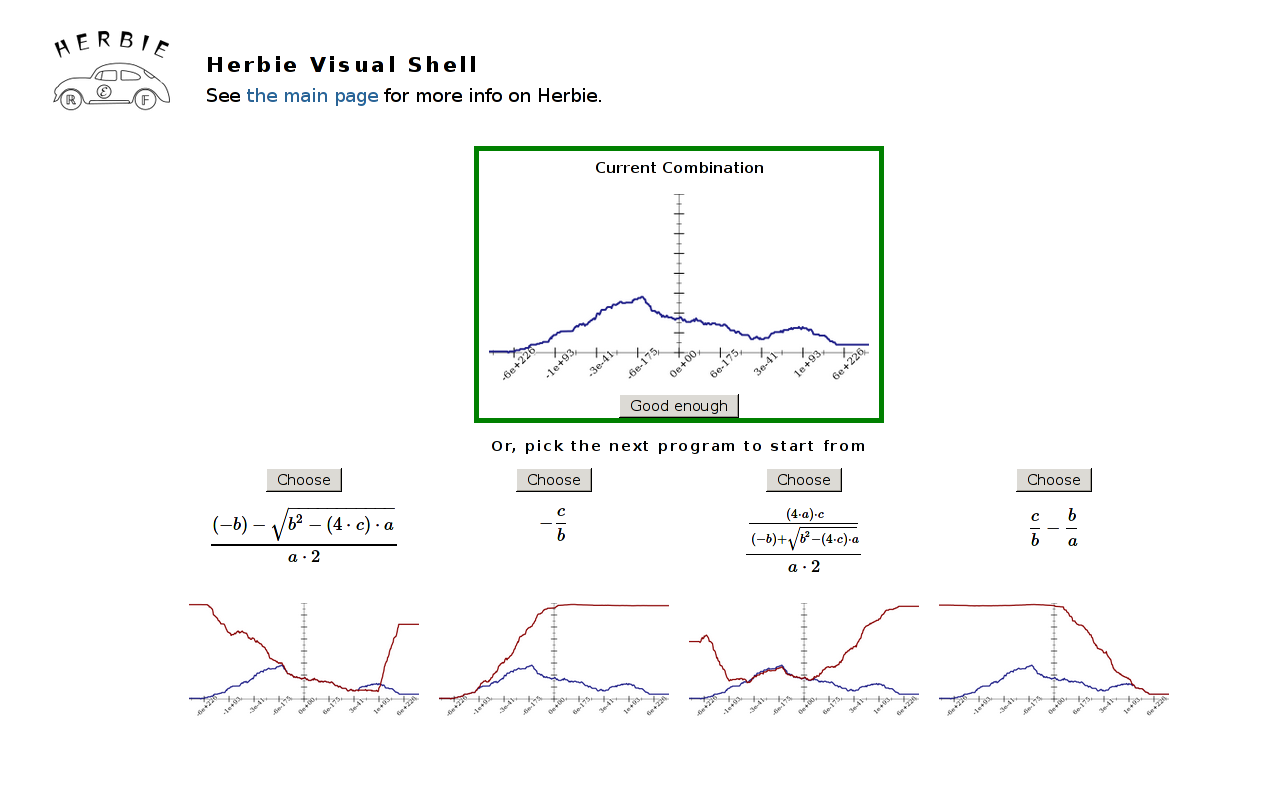
\includegraphics[width=.5\textwidth]{../../images/select_next_screen.png}
  \caption{The third phase of improvement. Here the user has just
    added new candidates by rewriting an existing candidate. The user
    is shown the error best combination of the candidates chosen so
    far, as well as all the individual candidates and how they compare
    to it. From here the user can go to the final program, or go back
    to phase one choosing another one of these programs as a base, to
    try to expand their group of chosen candidates.}
  \label{fig:select-next}
\end{figure}

\begin{figure}
  \centering
  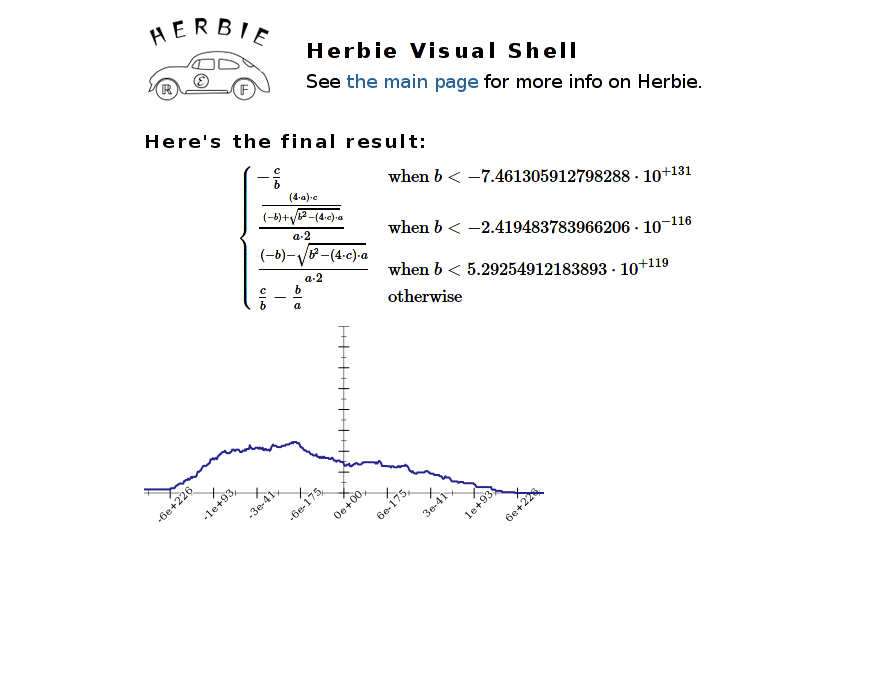
\includegraphics[width=.5\textwidth]{../../images/final_combo_screen.png}
  \caption{The final output program. These branches are computed
    with a higher number of samples points than the intermediary
    combinations, to ensure that the branch values are accurate. The
    final error graph is shown so that the user can assess if this
    program meets their needs. The user can then translate this
    formula into code in their program, which will accurately
    compute their formula.}
  \label{fig:final-combo}
\end{figure}

The Herbie Interactive Visualization is split into five distinct
``phases'', of which the first allows the user to enter their formula
and start the process, the middle three can be repeated to improve the
floating point implementation, and the last displays the final
implementation of the formula that the user provided.

In the first phase, the user is presented with a simple box for
entering the formula they want to improve (see
Figure~\ref{fig:enter-formula}). The user can enter any formula
involving arithmetic, exponentiation, and several trancendental and
trigonometric functions, modulo bugs in the current Herbie
implementation. These formulas are parsed into s-expressions
client-side by MathJS, and sent to the server to begin the improvement
session.

In the second phase, the user is shown a formatted version of the
formula they entered, and a graph of it's error (see
Figure~\ref{fig:select-loc}). The graph is generated according to the
process described in Section~\ref{sec:methods}. Operations which cause
significant amounts of error in the program are circled. The ranges
for the chosen input variable which have high error due to the
aforementioned operations are highlighted, with one highlight color
corresponding to each operation. Mousing over any location in the
displayed formula indicates it's corresponding ranges, and clicking on
an operation selects it and goes to the next phase.

In the third phase, the user is presented with a group of three or
less candidates generated by Herbie in response to the chosen location
(see Figure~\ref{fig:select-children}). These candidates are displayed
with the steps to generate them, and a graph comparing their error to
the error of the program they were generated from. In subsequent
iterations their error is compared to the best combination found so
far. The user can select number of the candidates to keep, and press
accept to progress to the next phase.

In the final improvement phase, the Herbie Interactive Visualization
infers the best branching combination of all the programs the user has
kept so far, and displays the error graph of this combination (see
Figure~\ref{fig:select-next}). Underneath are displayed the error
graphs of all the programs that the user has kept, compared to the
combination found. The user can compare each candidate to see how it
fits into the broader combination. Then, the user can either select a
particular candidate, returning to the first phase of improvement,
phase two, or they can progress onto the final phase. If they continue
to improve, all their candidates are kept, and new candidates add to
their group.

Finally, in the last phase, the branches are recomputed using more
points for higher accuracy, and the user is presented with the final
program, and a graph of its error (see
Figure~\ref{fig:final-combo}). The user can use this final error graph
to assess how useful the program is for their application, and can
transcribe the final output into their code.
\section{Discussion}
\label{sec:discussion}
While this visual interface was originally intended to help users
better diagnose and understand floating point issues as well as
Herbie's approach to solving them, it actually ended up helping the
development team of Herbie, including myself, understand more about
Herbie in a few key ways.

Firstly, by creating a friendly interface through which many users
could easily interact with Herbie, it allowed us to get valuable usage
data that we were previously unable to get. This revealed several bugs
and crashes in the Herbie software which we are now able to
address. In particular, a user when trying the tool replaced the
square root in the example formula, the quadratic formula, with a cube
root, and it triggered unintended behavior in Herbie which crashed the
session. Another user was able to compose a formula involving several
transcendental functions which also crashed the session. We were
previously unaware of these vulnerabilities in Herbie, and by exposing
it to a larger audience through a friendlier interface, we are now
able to address them.

Secondly, using the interface to navigate Herbie's improvement process
revealed several interesting things about the behavior of Herbie. In
the aforementioned quadratic formula example, there are two separate
sources of error: catastrophic cancellation in the numerator, and
overflow due to squaring $b$. The overflow is mitigated by Herbie
using two series expansions, chosen depending on whether the input
value of $b$ is very small or very large. For quite a while we
believed that Herbie was finding these series expansion by focusing on
the squaring operator, and then generating the series expansion which
fixed it's error. By interactively directing the improvement process
using the visual interface, we discovered that in actuality, Herbie
focuses on the subtraction, and discovers the series expansions which
fix the overflow quite by accident.

\section{Future Work}
\label{sec:future-work}

While the tool is useful as it exists, and has already helped us
better understand the Herbie system, there are still more improvements
that could be made.

Most of the substantial improvements are in the ways in which we
visually display the error of different candidate programs. Currently,
the system will attempt to find a single input variable which
accurately captures the error behavior of the program. While this
works on every example we have come across, there is no reason to
believe that there could not exist formulas for which there are
multiple accuracy issues due to different input variables. This could
be addressed either by finding and equally useful way to display the
error on multiple axis at once, by dynamically switching which axis is
displayed in response to different accuracy problems during the course
of improvement.

The current mechanism for tying locations of error to regions of the
input space is functional, and generally approximately correct, but it
has much variation and does not always behave as would be
expected. Further exploring algorithms to determine the clusters of
``bad'' error due to a certain operation could in the future be
explored.

Additionally, there are several input regions which are affected by
multiple errant operations. Instead of having a binary distinction
where regions are either negatively affected by a operation or not
negatively affected by an operation, it would be interesting to
explore visual ways to portray what proportion of the error is due to
what operations. This would particularly challenging since the error
due to different operations is not additive, and in fact the
relationship of the total error to the individual operation errors can
be as complex as the input formula itself.

Finally, the system could be smoothed and polished to make it easier
to interact with, by adding loading animations and improving click
detection on locations.

\bibliographystyle{abbrv}
\bibliography{references}

\end{document}
